\label{part_iaas}
\part{Infrastrucuture as a Service -- IaaS}

%%%%%%%%%%%%%%%%%%%%%%%%%%%%%%%%%%%%%%%%%%%%%%%%%%%%%%%%%%%%%%%%%%%%%%%%%%%
\begin{frame}
\frametitle{IaaS}
\framesubtitle{Components}
\begin{columns}
\column{.3\textwidth}
\begin{itemize}
\item Images
\item Instances
\item Block storage
\item Object storage
\item Network
\end{itemize}
\column{.7\textwidth}
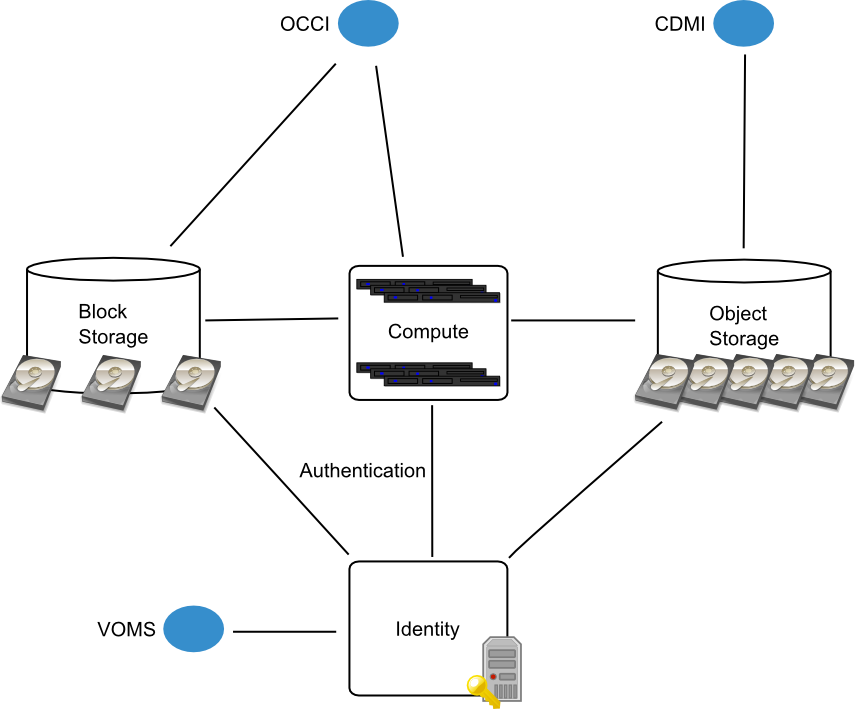
\includegraphics[width=\textwidth]{images/IaaS_OCCI.png}
\end{columns}
\end{frame}

%%%%%%%%%%%%%%%%%%%%%%%%%%%%%%%%%%%%%%%%%%%%%%%%%%%%%%%%%%%%%%%%%%%%%%%%%%%
\begin{frame}
\frametitle{IaaS}
\framesubtitle{What is an image?}
There are various answers to this question
\begin{itemize}
\item Typically
  \begin{itemize}
  \item A blob of data representing the contents of a disk or file system
  \item Usually contains the root file system contents of an operating system
  \end{itemize}
\item Application data can be conveyed within images
\item Image is usually used as a term for a \emph{template} to create
  a virtual machine or \emph{instance} of it.
  \begin{itemize}
  \item In OCCI terms, an image is an \emph{Operating System Template
    -- OS Template}
  \end{itemize}
%% another wonderful diagram showing the relations among image and instance
%% will add additional relations later on, e.g. block storage volumes
\end{itemize}
\end{frame}

%%%%%%%%%%%%%%%%%%%%%%%%%%%%%%%%%%%%%%%%%%%%%%%%%%%%%%%%%%%%%%%%%%%%%%%%%%%
\begin{frame}
\frametitle{IaaS}
\framesubtitle{What is an instance?}
\begin{itemize}
\item A virtual machine (VM)
  \begin{itemize}
  \item ... created from an \emph{image}
  \item ... given an amount of \emph{resources}
  \item ... and additional parameters (aka. \emph{user-data})
  \end{itemize}
\item User data is used to pass parameters to the instance
  \begin{itemize}
  \item This is used in the \emph{contextualization} process
  \item More details on this \hyperlink{part_contextualization}{later}
  \end{itemize}
\end{itemize}
\end{frame}

%%%%%%%%%%%%%%%%%%%%%%%%%%%%%%%%%%%%%%%%%%%%%%%%%%%%%%%%%%%%%%%%%%%%%%%%%%%
\begin{frame}
\frametitle{IaaS}
\framesubtitle{Storage}
Storage usually comes in two flavors
\begin{itemize}
\item Block Storage
  \begin{itemize}
  \item Can be attached to VM instances as block devices
  \item Transparent to applications running within VM
  \item Used to store data persistently (until the block device is deleted)
  \end{itemize}
\item Object Storage
  \begin{itemize}
  \item Accessible from anywhere (within and outside VMs)
  \item Virtually infinitely scalable
  \item Standard to access: CDMI
  \end{itemize}
\item More details on storage \hyperlink{part_storage}{later}
\end{itemize}
\begin{tikzpicture}
  \node at (10,5.5) [absolute,overlay] {\pgfimage[width=3cm]{images/DBaaS.png}};
  \node at (10,1.5) [absolute,overlay] {\pgfimage[width=3cm]{images/Object_Storage_Relations.png}};
\end{tikzpicture}
\end{frame}

%%%%%%%%%%%%%%%%%%%%%%%%%%%%%%%%%%%%%%%%%%%%%%%%%%%%%%%%%%%%%%%%%%%%%%%%%%%
\begin{frame}
\frametitle{Network}
Network as a resource, or Software Defined Networks (SDN) do not (yet) play a role in the EGI Federated Cloud.

\vspace{1em}
However
\begin{itemize}
\item At some sites users need to explicitly add public IP addresses
  to instances to make the available to the world
\item This can be achieved through the OCCI interface.
\end{itemize}
\end{frame}

%%% Local Variables:
%%% TeX-master: "2014-05-23_Best_Practices"
%%% End:
